\documentclass[tikz]{standalone}
\usepackage{tikz, mathrsfs, mathtools}
\usetikzlibrary{arrows, backgrounds}

\definecolor{vermelho}{RGB}{216,140,154}
\definecolor{verde}{RGB}{153,193,185}
\definecolor{azul}{RGB}{142,125,190}
\definecolor{amarelo}{RGB}{203,200,123}

\begin{document}

\def \dd {.05}
\def \d {.1}
\begin{tikzpicture}[scale=2.3, auto, swap]
    
    % chemical reactions and reservoirs
    \node at (-.6,.72) {(a)};
    \begin{scope}[shift={(0.3,0)}]
        \fill[rounded corners=1pt, fill=azul] (-.7, .5) rectangle ++(.6, .2) {};
        \fill[rounded corners=1pt, fill=verde] (-.7, -1.1) rectangle ++(.6, .2) {};
        \node at (-.4, .6) {A};
        \node at (-.4, -1) {B};
    
        \draw [->,azul] (-.4+0.02,.45) to (-.4+0.02,.3);
        \draw [<-,azul] (-.4-0.02,.45) to (-.4-0.02,.3);
        \draw [->,verde] (-.4+0.02,-.85) to (-.4+0.02,-.7);
        \draw [<-,verde] (-.4-0.02,-.85) to (-.4-0.02,-.7);
        
        \node at (-.4,.1) {\(A \xrightleftharpoons[k_{-1}]{k_1} X\)};
        \node at (-.4,-.2) {\(B \xrightleftharpoons[k_{-2}]{k_2} Y\)};
        \node at (-.4,-.5) {\(2X+Y \xrightleftharpoons[k_{-3}]{k_3} 3X\)};
    \end{scope}

    % state space
    \node at (.5,.72) {(b)};
    \begin{scope}[xscale=1,shift={(.8,-.9)}]
        \draw (-.1-\d,0) -- (1.5,0);
        \node at (1.2, -.1) {$X$};
        \draw (0-\d,-.1) -- (0-\d,1.5);
        \node at (-.1-\d, 1.4) {$Y$};

        \foreach \i in {.2,.7,1.2}{
            \draw[gray] (.1, \i) -- (1.8, \i);
            \draw[gray] (\i, .1) -- (\i, 1.4);
        }

        \draw[gray] (.2-\dd,1.2+\dd-.5) -- (1.2+\dd-.5,.2-\dd);
        \draw[gray] (.2-\dd,1.2+\dd) -- (1.2+\dd,.2-\dd);
        \draw[gray] (.2-\dd+.5,1.2+\dd) -- (1.2+\dd+.5,.2-\dd);
        \draw[gray] (.2-\dd+1,1.2+\dd) -- (1.2+\dd+.5,.2-\dd+.5);

        \begin{scope}[transparency group, opacity=0.75]
            \draw[thick, azul!90!black, ->, line width = .7mm] (.7,.2) -- node[anchor = north] {$-_A$} (.2,.2);
            \draw[thick, verde!90!black, ->, line width = .7mm] (.2,.2) -- node[anchor = east] {$+_B$} (.2,.7);
            \draw[thick, vermelho!90!black, ->, line width = .7mm] (.2,.7) -- node[anchor = south, sloped] {inner} (.7,.2);
        \end{scope}

        \foreach \i in {0,.5}{ \node at (.35+\i,.35) {$\Delta\mu$};}
        \foreach \i in {0,.5}{ \node at (.35+\i,.85) {$\Delta\mu$};}
        
    \end{scope}

    \node at (3,-.27) {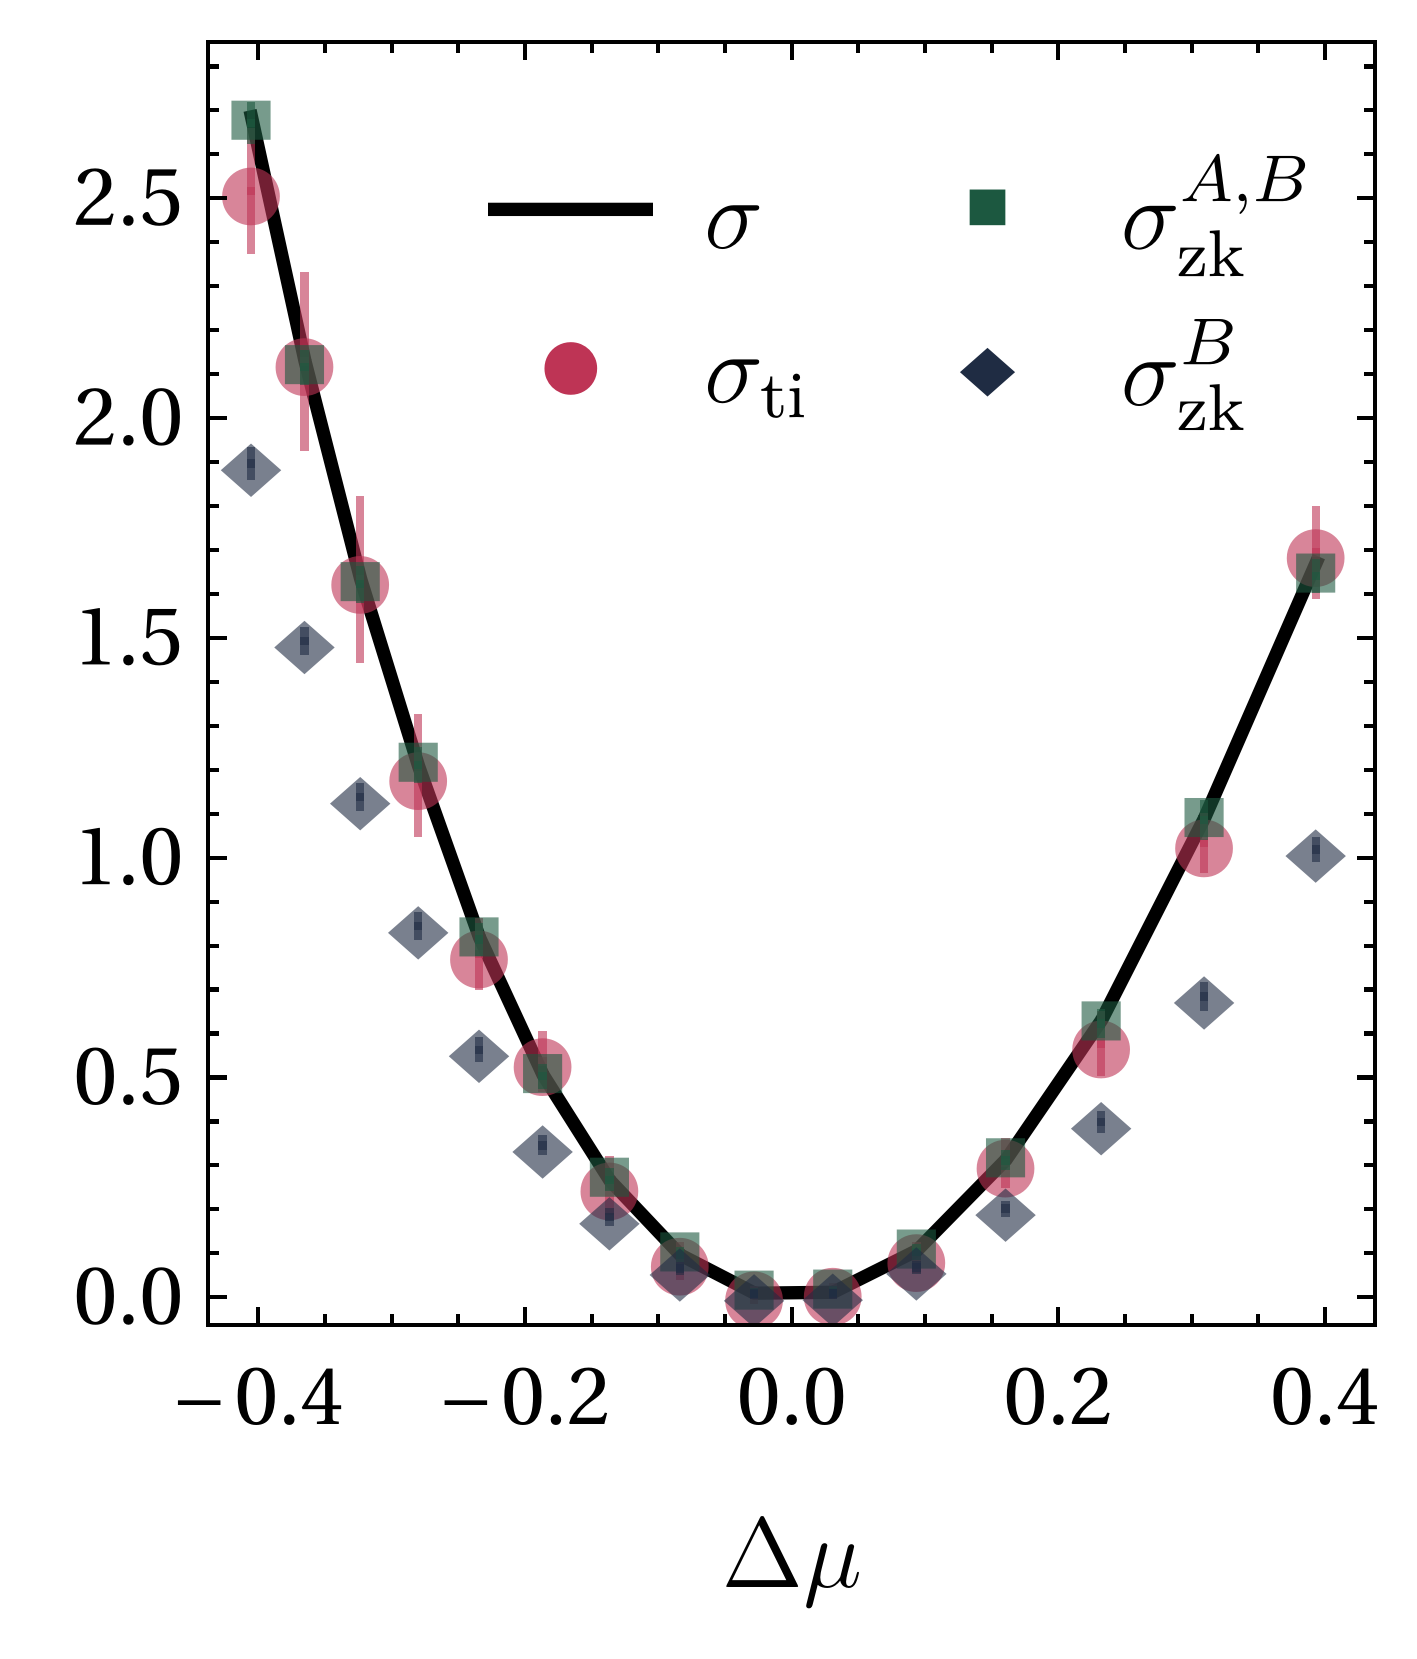
\includegraphics[width=0.35\textwidth]{plot_Bruss_EPR.png}};
    \node at (2.1,.72) {(c)};
    
    \node at (4.86,-.27) {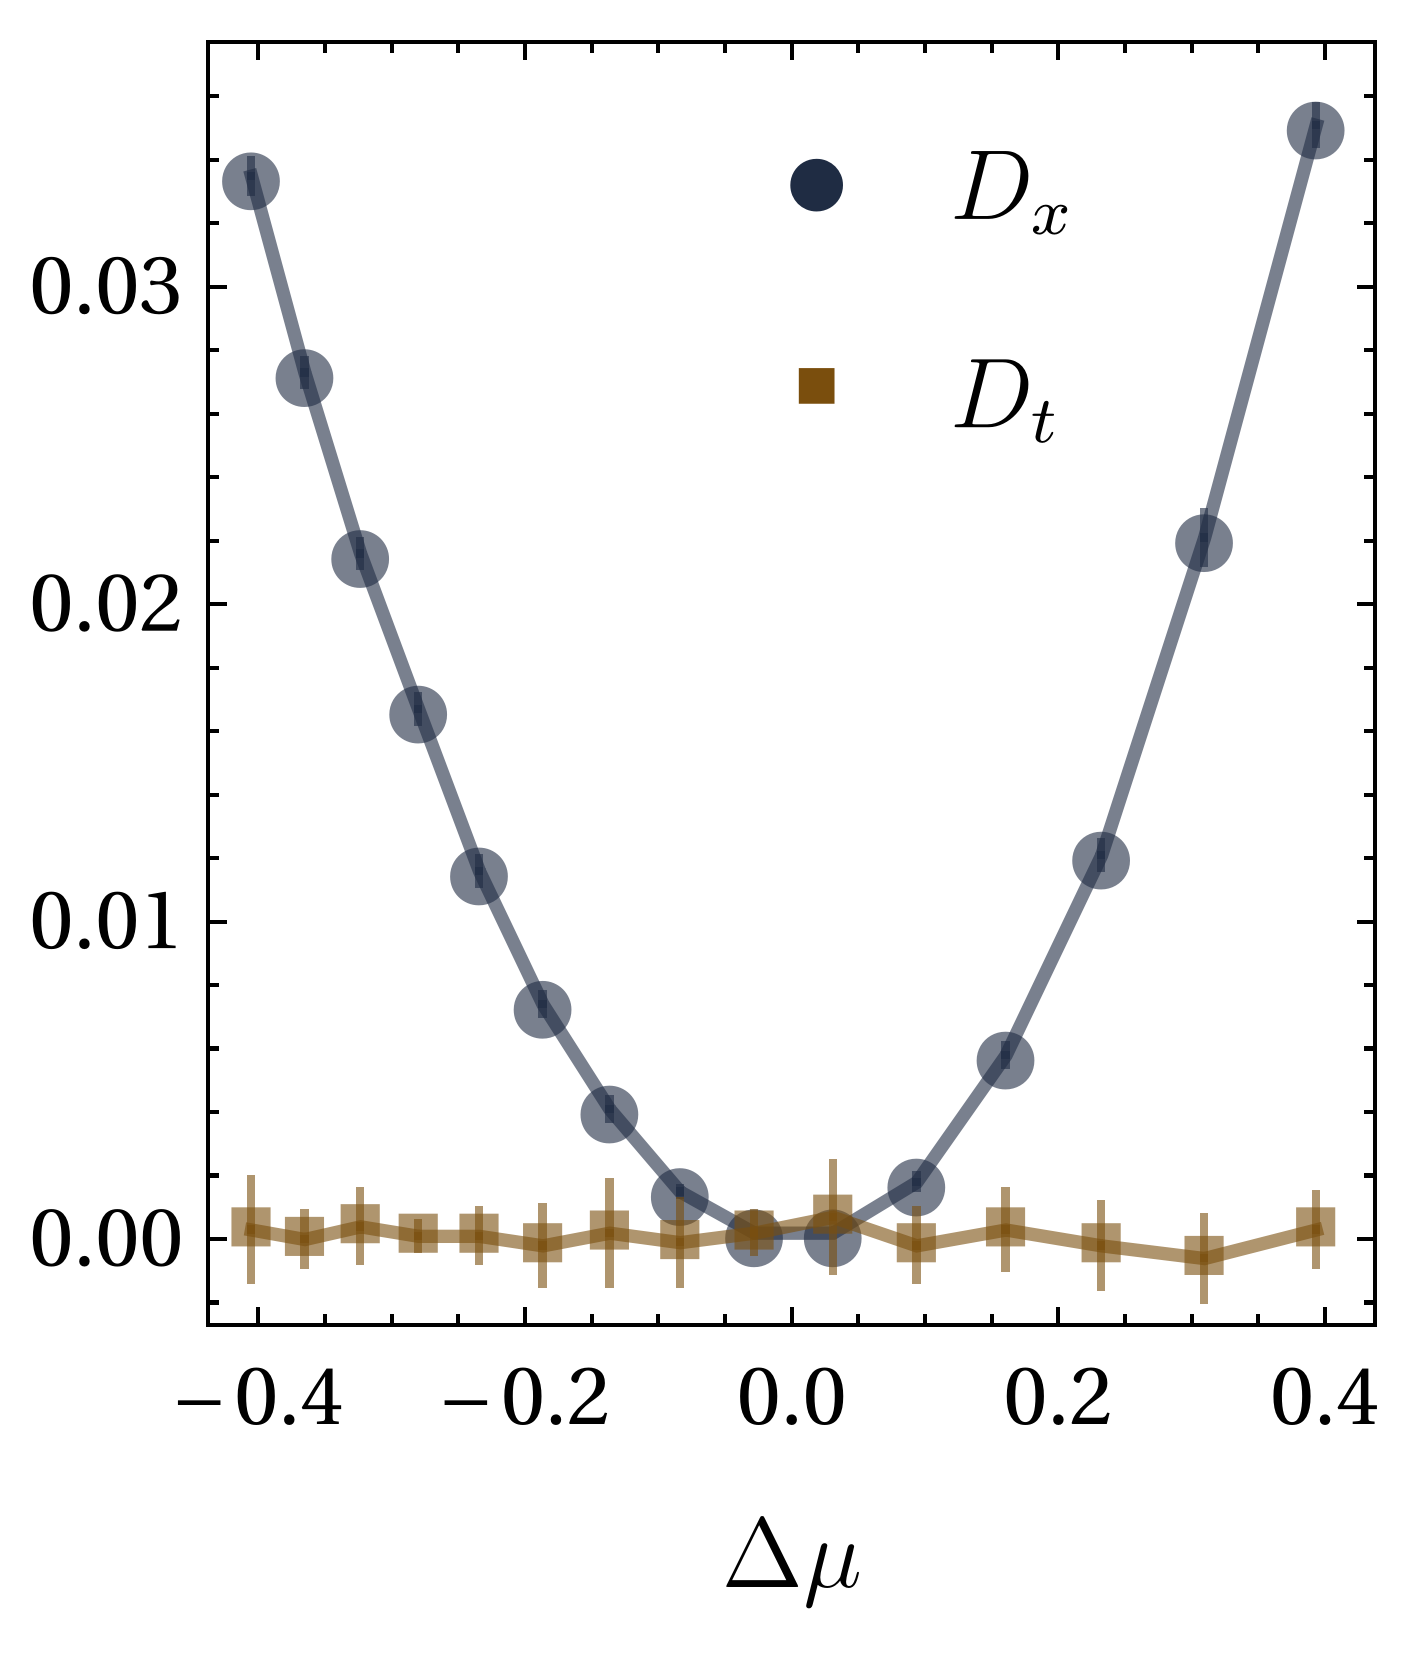
\includegraphics[width=0.35\textwidth]{plot_Bruss_Dxt.png}};
    \node at (4,.72) {(d)};
    
\end{tikzpicture}


\end{document}
